\chapter{Resultados}
\label{chapter:resultados}

Con el objetivo de evaluar si la nueva versión de \gls{feets} logra efectivamente mitigar las limitaciones identificadas en su versión original, realizamos una evaluación exhaustiva centrada tanto en el desempeño computacional como en la calidad estructural del código.

Por un lado, analizamos los tiempos de ejecución del sistema bajo distintas configuraciones experimentales, con el fin de determinar el impacto de la paralelización y la incorporación de nuevas funcionalidades. Por el otro, examinamos la evolución de la mantenibilidad del código mediante técnicas de análisis estático, con el propósito de cuantificar los efectos de las mejoras implementadas en términos de calidad. A continuación, presentamos en detalle los análisis realizados y los resultados obtenidos.

\section{Comparación de tiempos de ejecución}

Para evaluar el desempeño del nuevo modelo de extracción paralelizado, medimos sistemáticamente los tiempos de ejecución del proceso de extracción de características a lo largo de una serie de experimentos controlados. En cada experimento, generamos aleatoriamente un conjunto de una o más \glspl{lc} periódicas, simuladas al azar, que luego utilizamos como entrada para el proceso de extracción. Repetimos las pruebas variando los siguientes parámetros:

\begin{enumerate}
    \item \textbf{Longitud:} Número total de observaciones en cada una de las \glspl{lc} simuladas. Las longitudes variaron entre 30, 100, 300 y 1000 observaciones.
    
    \item \textbf{Tamaño:} La cantidad de \glspl{lc} simuladas que se procesaron en simultáneo. Probamos con tamaños de 1, 50, 100, 500 y 1000 \glspl{lc}.

    \item \textbf{Estrategia:} La configuración utilizada por el \emph{scheduler} de \emph{Dask} para distribuir las tareas. Como mencionamos en el \autoref{chapter:parallel}, nos interesaron tres \emph{schedulers} preestablecidos: \texttt{synchronous} (sin paralelismo), \texttt{threads} (\emph{multithreading}) y \texttt{processes} (\emph{multiprocessing}). 
\end{enumerate}

Al combinar las distintas configuraciones de los tres parámetros, obtenemos 60 experimentos distintos. Para cada uno de ellos, realizamos diez iteraciones independientes, generando en cada repetición un nuevo conjunto de \glspl{lc} simuladas. En total, se llevaron a cabo 600 casos de prueba, en los cuales medimos el tiempo de ejecución del proceso completo de extracción en dos escenarios distintos:

\begin{enumerate} 
    \item \textbf{Selección completa:} Abarcando todas las características disponibles en la nueva versión de \gls{feets}, incluyendo las que incorporamos mediante la integración con \textit{LightCurve}. 
    
    \item \textbf{Selección reducida:} Limitada únicamente a las características que ya estaban presentes en versiones anteriores de la herramienta.
\end{enumerate}

Las mediciones fueron llevadas a cabo en la supercomputadora Serafín, provista por la \unc{}. Cada caso de prueba se ejecutó en una unidad de cómputo con las siguientes características:

\begin{description}
    \item[CPU] -- $\SI{2.4}{\giga\hertz}$ AMD EPYC\texttrademark{} 7532 ($2\times32$ núcleos, 64 hilos, $\SI{256}{\mega\byte}$ de caché, hasta $\SI{3.3}{\giga\hertz}$).
    \item[RAM] -- $\SI{128}{\gibi\byte}$ DDR4 SDRAM ($16 \times \SI{8}{\gibi\byte}$, $\SI{3200}{\mega\hertz}$).
    \item[OS] -- Rocky Linux 8.8 con Linux Kernel 4.18.
    \item[\emph{Software}] -- \textit{Python} 3.13.2, \textit{NumPy} 2.2.4, \textit{SciPy} 1.15.2, \textit{AstroPy} 7.0.1, \textit{StatsModels} 0.14.4, \textit{Dask} 2025.3.0 y \textit{Light\-Curve} 0.10.2.
\end{description}

\subsection{Análisis de resultados}

\begin{figure}[!ht]
\centering
\begin{subfigure}{\textwidth}
    \centering
    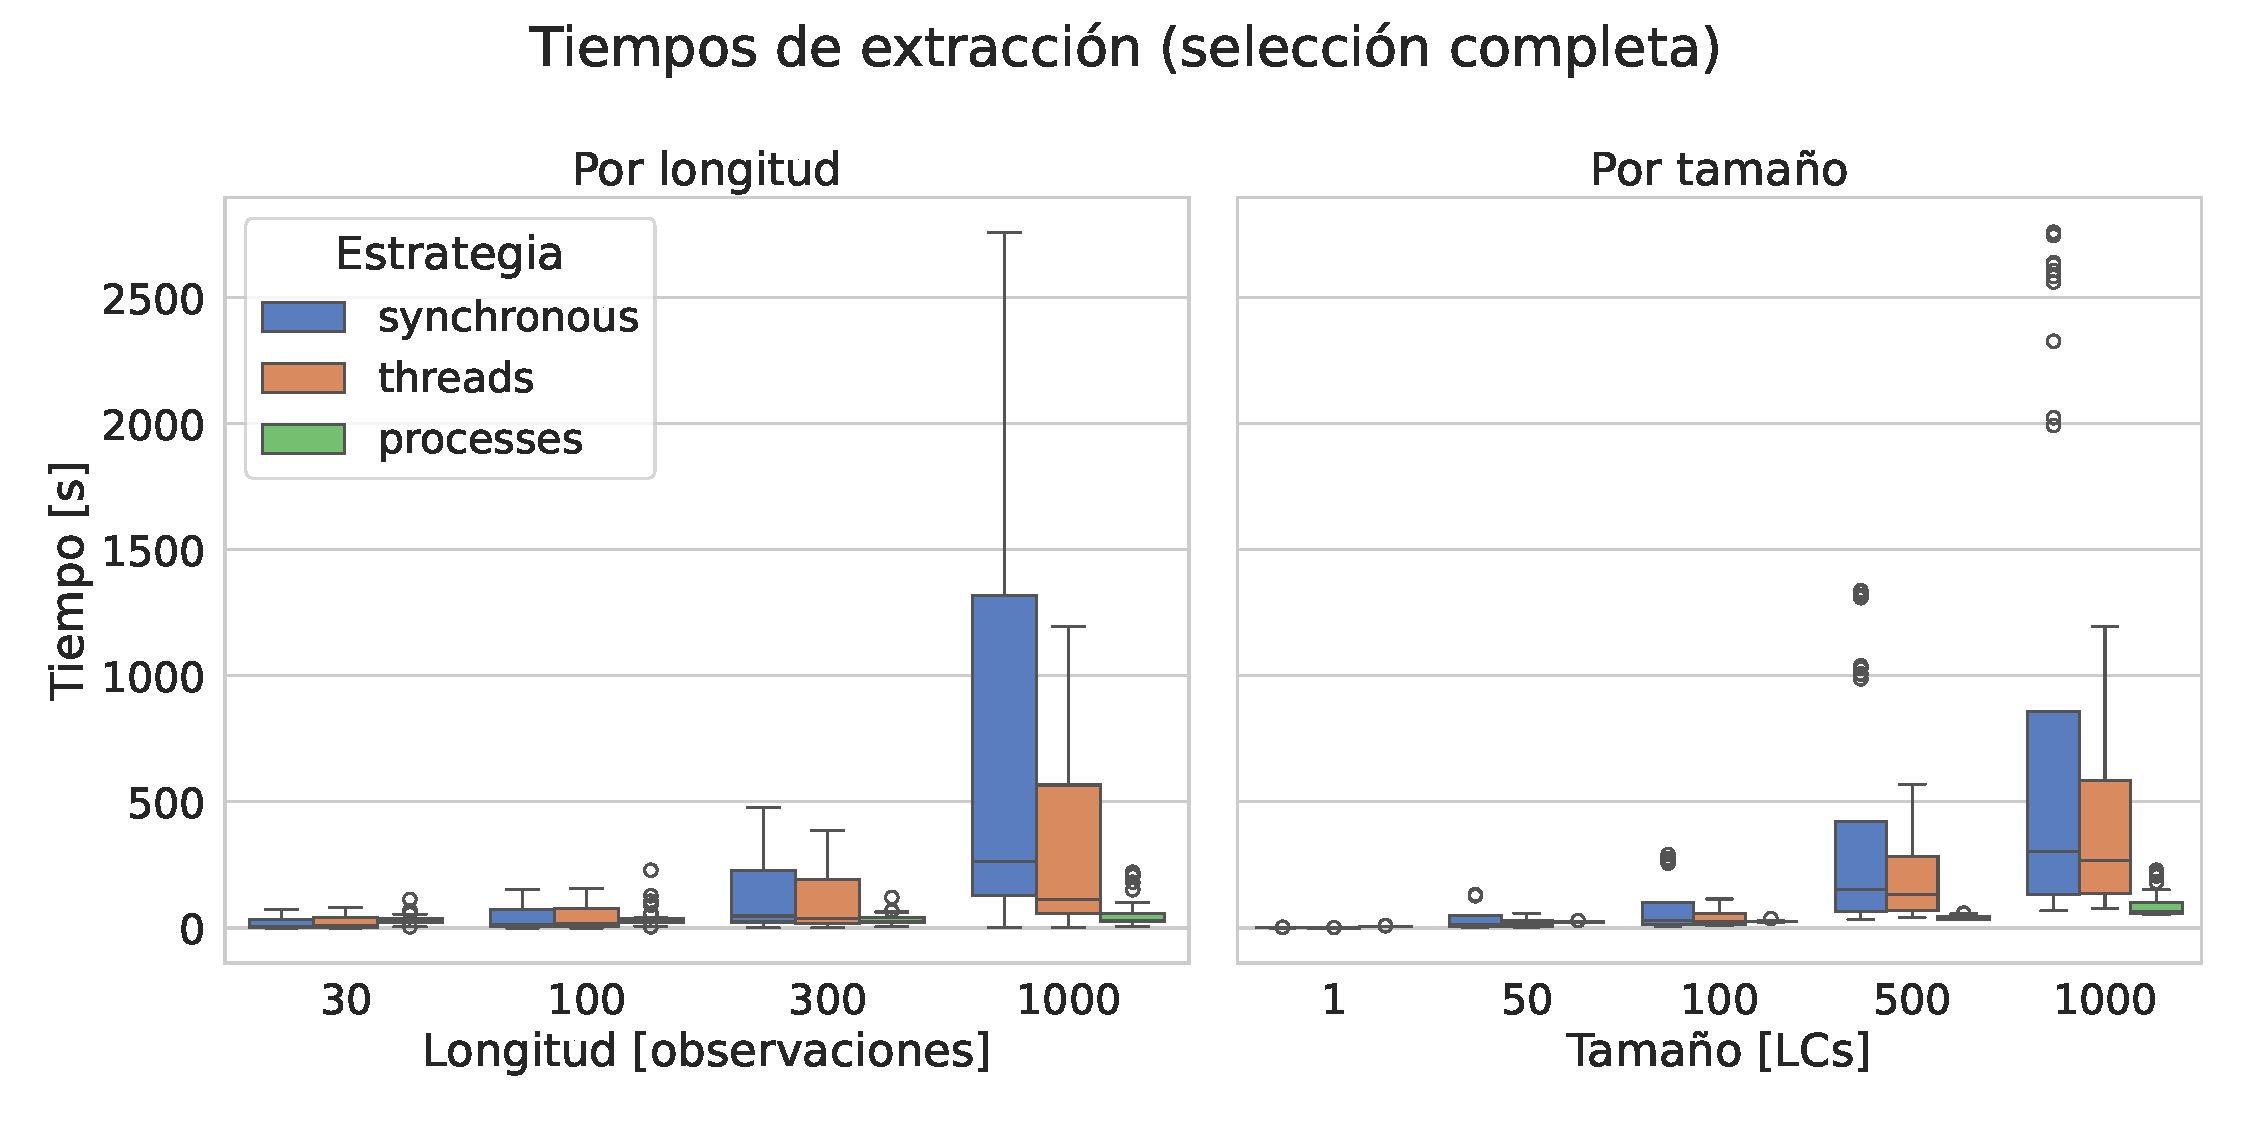
\includegraphics[width=\linewidth]{08_resultados/figures/01_analysis_all.pdf}
    \caption{Tiempos de extracción para la selección completa}
    \label{fig:analysis_all}
\end{subfigure}

\begin{subfigure}{\textwidth}
    \centering
    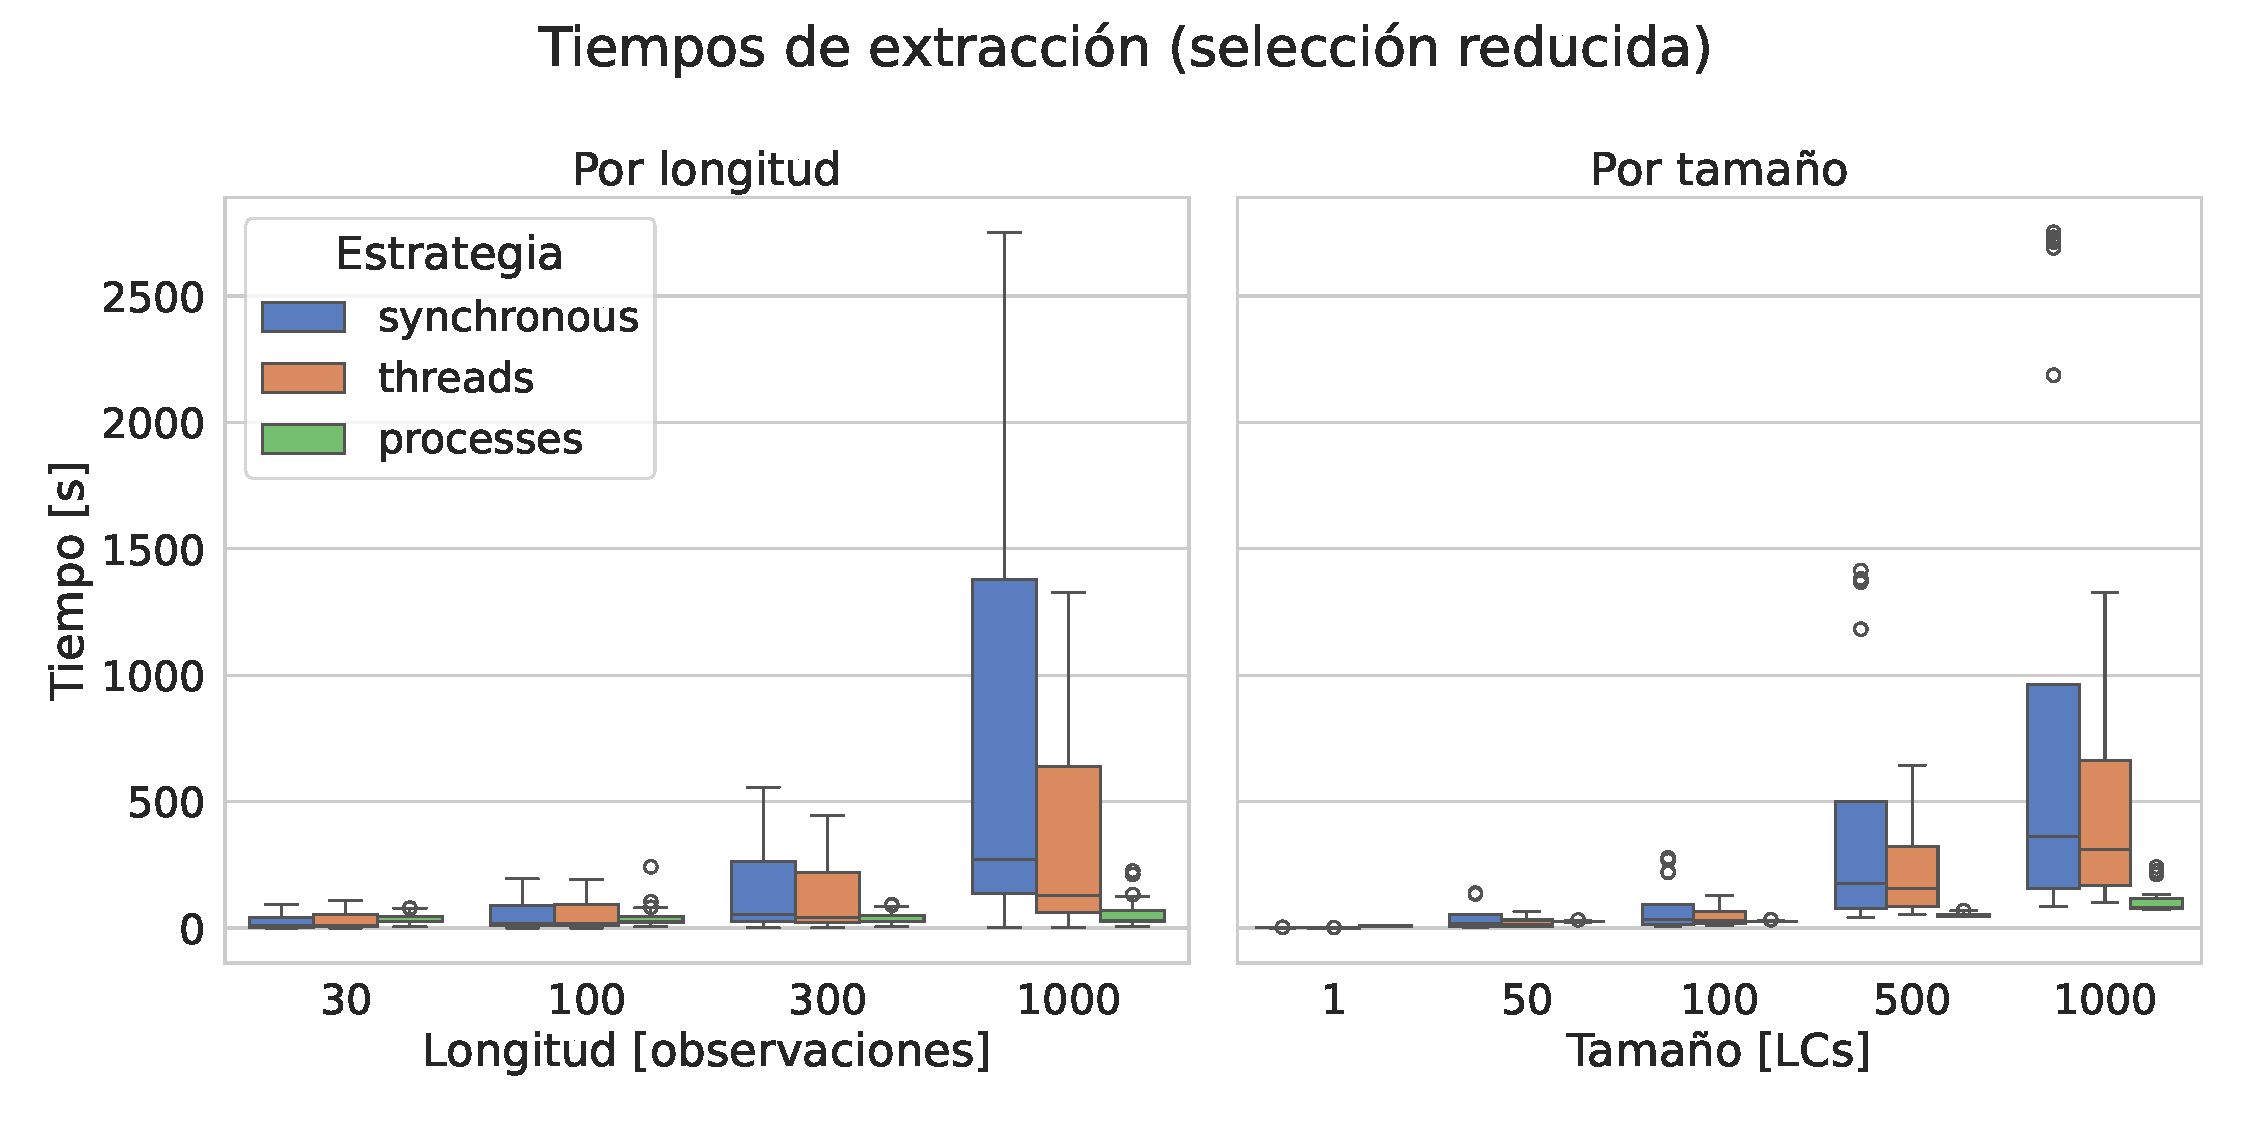
\includegraphics[width=\linewidth]{08_resultados/figures/01_analysis_exclude.pdf}
    \caption{Tiempos de extracción para la selección reducida}
    \label{fig:analysis_exclude}
\end{subfigure}

\caption{
    Evolución de los tiempos de extracción obtenidos para los 600 casos de prueba. Se visualizan dos conjuntos de gráficos por cada figura: uno en función a la longitud de las \glspl{lc} simuladas, y el otro en función a la cantidad de \glspl{lc} procesadas en simultáneo. Cada línea de color representa una estrategia del \emph{scheduler} de \emph{Dask} diferente.
}
 \label{fig:analysis}
\end{figure}

Los resultados obtenidos se resumen en las Figuras~\ref{fig:analysis_all} y~\ref{fig:analysis_exclude}, que presentan los tiempos correspondientes a la extracción tanto de todas las características del sistema como de la selección reducida, respectivamente. En términos generales, observamos que en los dos escenarios los tiempos de ejecución aumentan tanto con la longitud de las curvas como con el tamaño del conjunto. Esta relación era esperable, ya que un mayor volumen de datos implica un mayor esfuerzo computacional.

Al observar el comportamiento de las distintas estrategias de planificación, notamos que en los casos de menor volumen de datos (tanto el de menor longitud de observaciones como el de menor cantidad de \glspl{lc}) todas las estrategias muestran un rendimiento muy similar. En particular, \texttt{synchronous} suele ser ligeramente más rápida en esos escenarios, posiblemente porque los costos asociados a la creación, distribución y comunicación de tareas paralelas superan los beneficios del paralelismo en situaciones de baja carga. A medida que el volumen de los datos aumenta, \texttt{synchronous} muestra una tendencia clara a producir tiempos de ejecución progresivamente más altos, estableciéndose como la estrategia que peor escala. Este comportamiento evidencia la idea de que el paralelismo contribuye de manera efectiva a reducir los tiempos de extracción en contextos con mayor demanda.

Si nos centramos ahora en las dos estrategias concurrentes, observamos que \texttt{threads} presenta una mejora clara respecto de \texttt{synchronous}, especialmente en configuraciones de carga media. No obstante, \texttt{processes} demuestra ser consistentemente más eficiente que \texttt{threads}, con una ventaja considerable cuando la carga de datos es más elevada. Esta diferencia sugiere que el \emph{multiprocessing} permite un uso mucho más efectivo de los recursos disponibles con respecto al \emph{multithreading}, probablemente al evitar las limitaciones impuestas por el \gls{gil} de Python.

Cabe señalar que Dask ofrece otros \emph{schedulers} además de los tres evaluados, incluyendo el \texttt{distributed}, un planificador altamente configurable que permite ejecutar tareas en clústeres de múltiples máquinas o entornos con recursos heterogéneos. Explorar el comportamiento del sistema bajo esta configuración podría resultar especialmente interesante para escenarios con grandes volúmenes de datos o requerimientos de alta disponibilidad, y constituye una posible línea de trabajo futura.

Ahora bien, al comparar los escenarios de extracción completa y reducida, notamos que los tiempos de ejecución son similares en todos los casos, pero que en algunas configuraciones la extracción completa muestra tiempos ligeramente menores. Este resultado es especialmente interesante, ya que ambos escenarios se probaron sobre los mismos conjuntos de \glspl{lc}, siendo la única diferencia entre los dos la selección de características extraídas.

Una posible explicación para la mejora de la extracción completa es que las nuevas características incorporadas provienen de la integración con \textit{LightCurve}, la cual implementa sus funciones internas de forma altamente optimizada. Es posible que la forma en que estas operaciones están estructuradas y que interactúan con el planificador de tareas de \emph{Dask} favorezcan a una mejor distribución de carga o a una ejecución más eficiente en paralelo. En ese sentido, aunque se estén calculando más características, el sistema podría estar aprovechando mejor los recursos disponibles gracias al diseño eficiente de la implementación subyacente.

En cualquier caso, las diferencias de tiempo entre los dos escenarios son mínimas y no permiten concluir que una configuración sea sistemáticamente más rápida que la otra, pero sí permiten afirmar que la inclusión de nuevas características no introduce un costo computacional significativo. El rendimiento del sistema se mantiene estable independientemente del conjunto de características utilizadas, lo que refleja una implementación robusta, eficiente y bien integrada.

\section{Análisis estático de código}

Además de optimizar el desempeño de \gls{feets} para la extracción de características, otro de los objetivos centrales de este trabajo fue mejorar la calidad interna del código, es decir, su claridad, modularidad y facilidad de mantenimiento. Para evaluar este aspecto, aplicamos un enfoque de análisis estático, centrado en el cálculo del \acrfull{mi} del sistema a lo largo del tiempo.

\subsection{Análisis de resultados}

Para realizar el análisis, optamos por la herramienta \emph{Wily}\footnote{\url{https://wily.readthedocs.io/en/latest/}}, una biblioteca de Python que permite monitorear la evolución histórica de distintas métricas de calidad del código fuente. \emph{Wily} analiza cada revisión en el historial de Git del proyecto, generando un seguimiento detallado de métricas de complejidad y de tamaño y, en particular, el \gls{mi}.

Como vimos en el \autoref{chapter:antecedentes}, existen varias formas distintas para determinar el \gls{mi}, pero este cálculo normalmente involucra cuatro métricas fundamentales:

\begin{itemize}
    \item Comlejidad ciclomática (\acrshort{cc})
    \item Volumen de Halstead (\acrshort{hv})
    \item Líneas de código (\acrshort{loc})
    \item Porcentaje de comentarios (\acrshort{poc})
\end{itemize}

En nuestro caso, \emph{Wily} utiliza internamente la biblioteca \emph{Radon}\footnote{\url{https://radon.readthedocs.io/en/latest/}} para determinar el \gls{mi}, cuyo cálculo se basa en las variantes del \gls{sei} \citep{bray1997c4} y la de Visual Studio \citep{microsoft2025mi} para obtener la siguiente fórmula: \[
    \max \Bigg[
        0, \;
        \frac{100}{171}
        \Big(
            171 - 5.2\ln{\text{V}} - 0.32\text{CC}
            - 16.2\ln{\text{LOC}} + 50 \sin{\sqrt{2.4 \text{POC}}}
        \Big)
    \Bigg]
\]
Este cálculo pondera negativamente la complejidad y el tamaño del código, y positivamente la presencia de comentarios, dejándolo en un rango de valores entre 0 y 100. Cuanto más alto sea el puntaje, mayor será la mantenibilidad del archivo.

Un aspecto técnico importante a mencionar es que la herramienta \emph{Radon}, por defecto, no considera las cadenas de documentación (\emph{docstrings}) como parte de los comentarios, sino que las contabiliza como líneas de código normales. Esto genera una disminución significativa del \gls{mi} en módulos bien documentados, lo cual resulta en una aparente contradicción: una mejora en la legibilidad y comprensión del código penaliza su mantenibilidad según el puntaje. Para resolver esta paradoja, optamos por configurar \texttt{radon} de modo que los \emph{docstrings} sean tratados como comentarios. Consideramos que esta decisión refleja de manera más justa el impacto positivo de la documentación sobre la calidad y sostenibilidad del sistema.

\subsection{Resultados y análisis}

\begin{figure}[!ht]
    \centering
    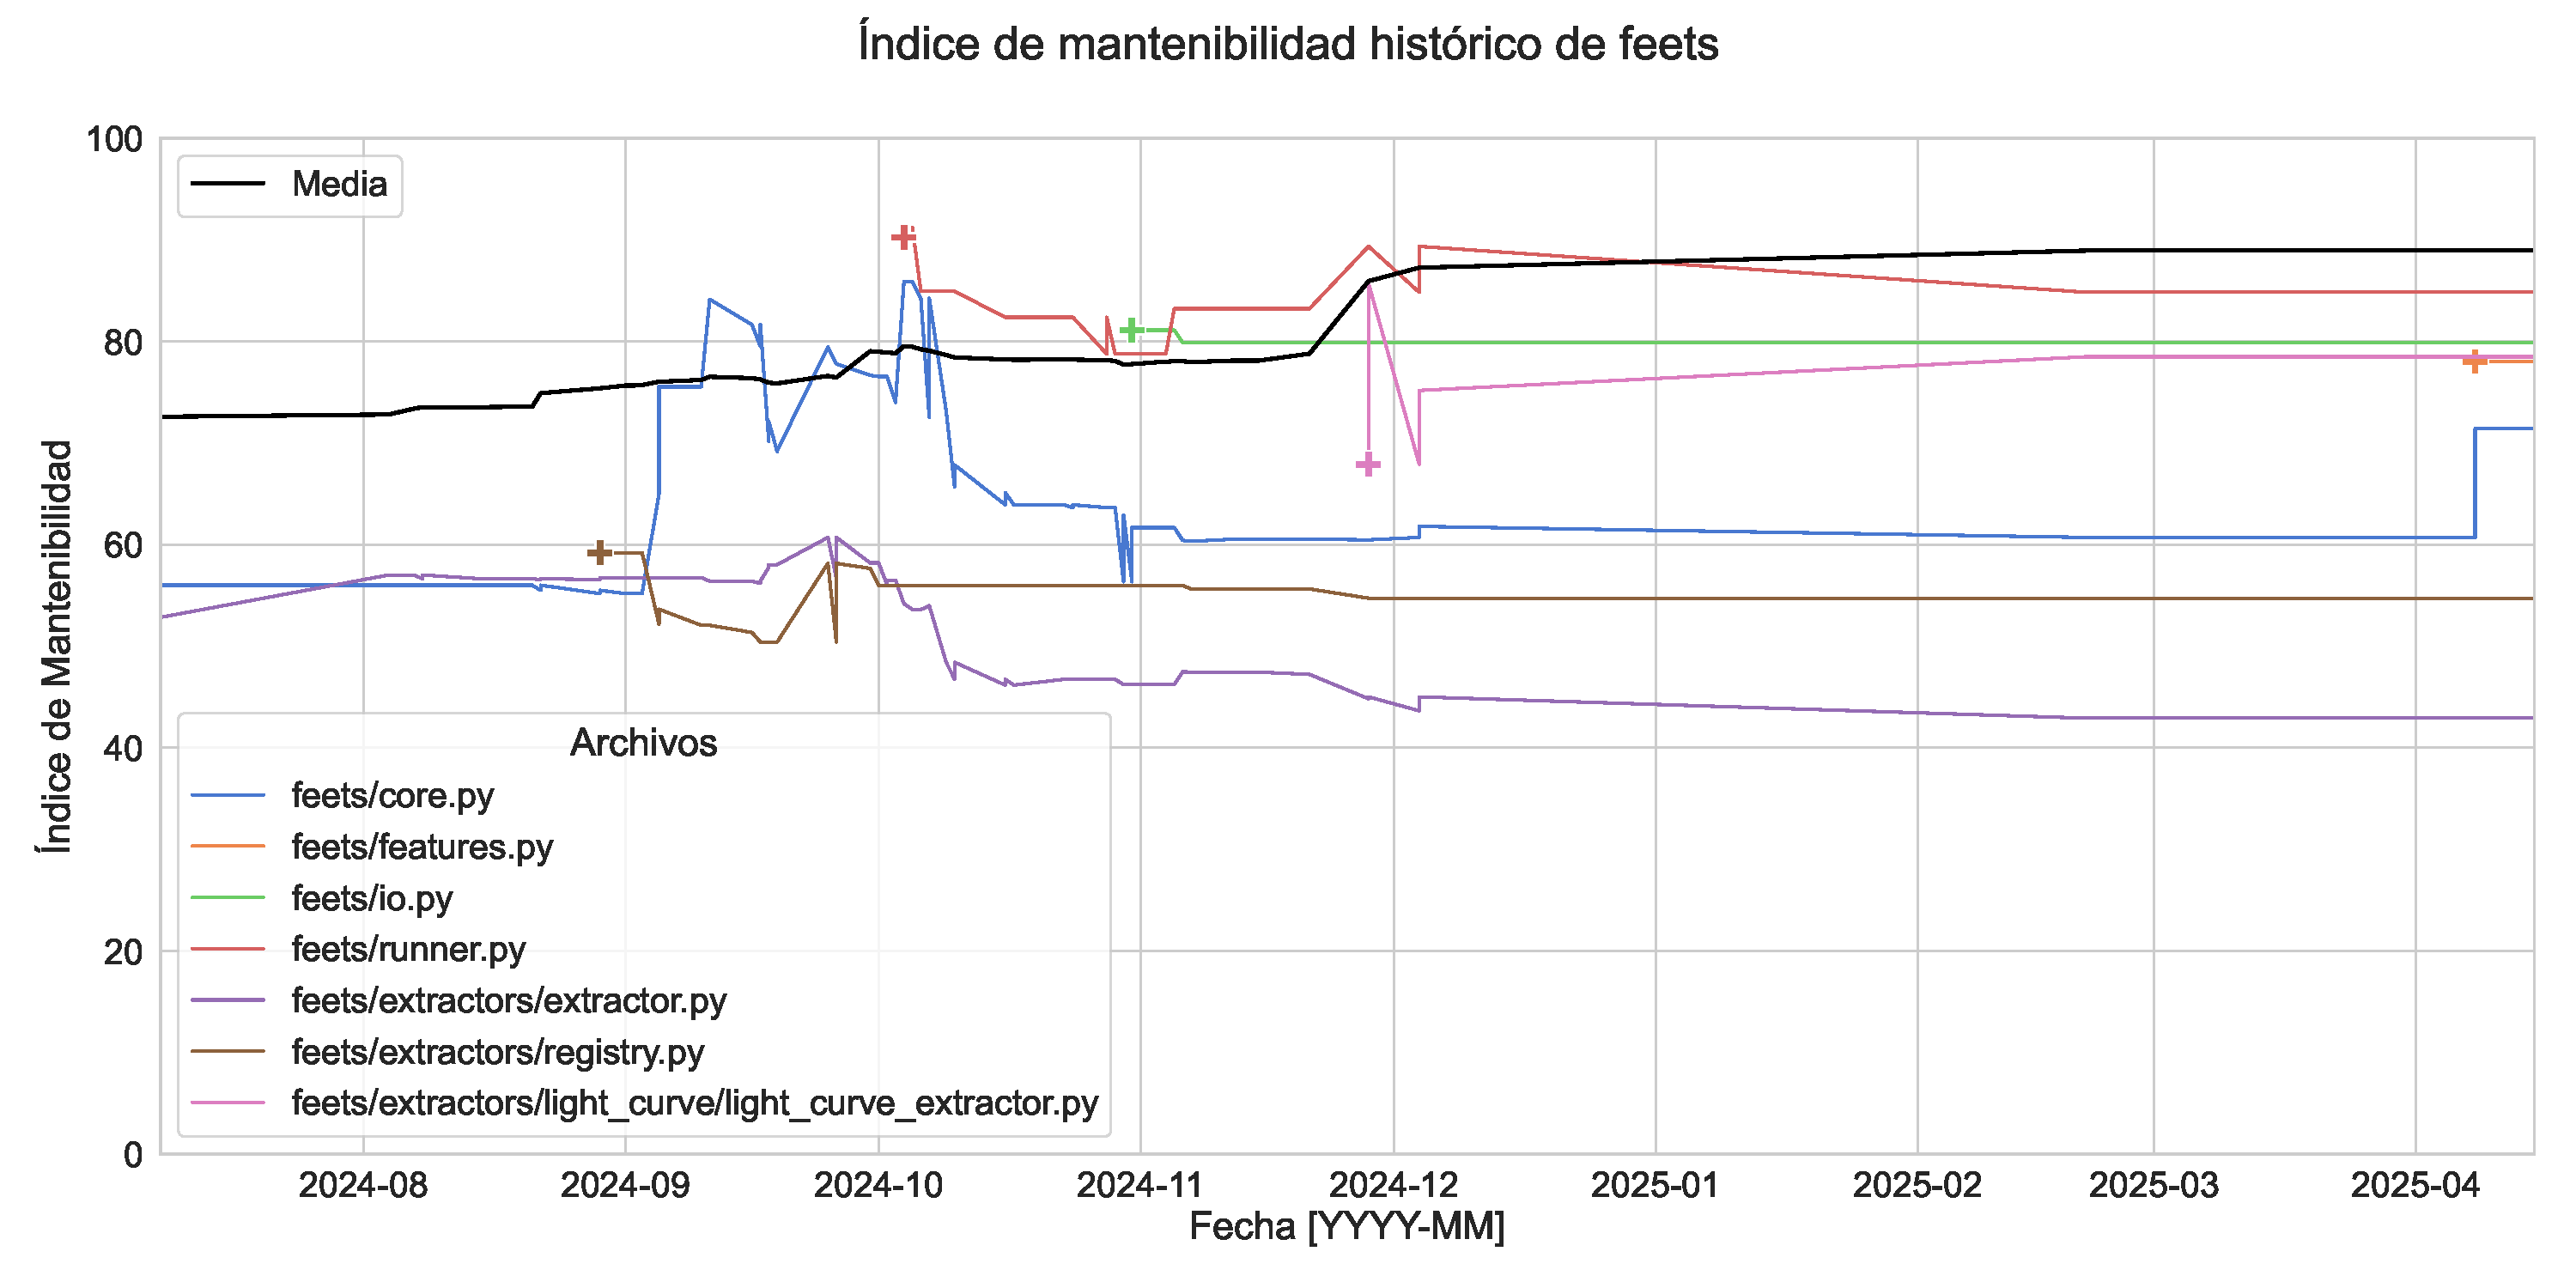
\includegraphics[width=\linewidth]{08_resultados/figures/MI_feets.pdf}
    \caption{
        Evolución del \gls{mi} de \gls{feets} durante el desarrollo de la nueva versión. La curva en negro representa la media del \gls{mi} considerando todos los archivos del sistema. Las líneas de colores, en cambio, muestran el \gls{mi} de algunos archivos individuales, seleccionados por su relevancia funcional, usando el símbolo \texttt{+} para marcar el momento en que se incorporaron al control de versiones.
    }
    \label{fig:mi}
\end{figure}

La \autoref{fig:mi} presenta la evolución del \gls{mi} a lo largo del proceso de modernización de \gls{feets}. Esta visualización permite identificar tendencias generales y también comportamientos específicos de ciertos módulos relevantes.

El valor medio del \gls{mi} global (representado por la curva negra) evidencia una ascendencia consistente en la mantenibilidad del sistema. Notamos un incremento de $72.59$ a $88.94$ puntos en el período analizado, reflejando una mejora sostenida en la calidad del código fuente de \gls{feets}. Desde una perspectiva técnica, este crecimiento puede atribuirse a prácticas de refactorización, modularización y reorganización de componentes, que derivaron en una base de código más clara y fácil de mantener.

Entre los archivos relevantes del proyecto, podemos notar algunas tendencias claras:

\begin{itemize}
    \item El módulo \texttt{feets/core.py} mostró un crecimiento destacado en su \gls{mi}; más aún, su curva muestra picos ascendentes en el momento en que se agregaron los módulos \texttt{feets/runner.py}, \texttt{feets/io.py} y \texttt{feets/features.py}. Este comportamiento es coherente con los cambios realizados en la nueva versión, pues gran parte de la lógica de \texttt{feets/core.py} fue externalizada a los módulos mencionados, sugiriendo que la separación de responsabilidades tuvo un impacto positivo en la mantenibilidad del código.

    \item En contraposición, el archivo \texttt{feets/extractors/extractor.py} experimentó una disminución gradual en su \gls{mi}. Esta tendencia también es esperable, ya que los nuevos extractores introdujeron funcionalidades adicionales, validaciones más complejas y capacidad de ejecución en paralelo, lo cual incrementó inevitablemente la complejidad del código y, por lo tanto, redujo su mantenibilidad.

    \item El archivo \texttt{feets/lightcurve/light\_curve\_extractor.py} mantuvo un \gls{mi} elevado desde su incorporación, lo cual sugiere que fue diseñado desde el inicio con buenas prácticas y una estructura clara. Este módulo actúa como puente entre los extractores de características de \gls{feets} y los de \textit{LightCurve}, por lo que su buen desempeño en términos de mantenibilidad indica que la integración fue realizada sin comprometer la calidad estructural del sistema.
\end{itemize}

A pesar de las variaciones individuales, el \gls{mi} se mantuvo en general en valores altos para los módulos relevantes, con puntajes superiores a los 60 puntos en la mayoría de los casos. Las excepciones más notorias fueron \texttt{feets/ex\-trac\-tors/re\-gis\-try.py} y \texttt{feets/extractors/extractor.py}, que mantuvieron puntajes más bajos y representan áreas donde aún queda margen de mejora en términos de claridad, modularidad y simplicidad estructural.

En conjunto, los resultados muestran que el sistema no solo creció funcionalmente, sino que lo hizo con una mejora tangible en su calidad interna. El análisis histórico del \gls{mi} permite afirmar que las decisiones de diseño y refactorización aplicadas durante el desarrollo tuvieron un impacto positivo en la mantenibilidad del código.

\section{Conclusiones del capítulo}

Juntando los resultados obtenidos a lo largo del capítulo, observamos que no solo la modernización de \gls{feets} llevó a mejoras significativas en los tiempos de ejecución de la herramienta, sino que también logró hacerlo sin comprometer la mantenibilidad global del sistema. En conjunto, estos hallazgos confirman que la nueva versión de \texttt{feets} representa un avance tanto en rendimiento como en calidad técnica.